\documentclass[12pt,a4paper]{article}

%%%%%%%%%%%%%%%%%%%%%%%%%%%%%%%%%%%%%%%%%%%%%%%%%%%%%%%%%%%%%%%%%%%%%%%%%%%%%%%
% HEADERS
%%%%%%%%%%%%%%%%%%%%%%%%%%%%%%%%%%%%%%%%%%%%%%%%%%%%%%%%%%%%%%%%%%%%%%%%%%%%%%%
\usepackage[utf8]{inputenc}
\usepackage[greek,english]{babel}
\usepackage{alphabeta} 
\usepackage{amsmath}
\usepackage{algorithm} 
\usepackage{algpseudocode} 

\usepackage[pdftex]{graphicx}
\graphicspath{ {./images/} }
\usepackage[top=1in, bottom=1in, left=1in, right=1in]{geometry}
\usepackage{float}

\linespread{1.06}
\setlength{\parskip}{8pt plus2pt minus2pt}

\widowpenalty 10000
\clubpenalty 10000

\newcommand{\eat}[1]{}
\newcommand{\HRule}{\rule{\linewidth}{0.5mm}}

\usepackage[official]{eurosym}
\usepackage{enumitem}
\setlist{nolistsep,noitemsep}
\usepackage[hidelinks]{hyperref}
\usepackage{cite}


\begin{document}

%%%%%%%%%%%%%%%%%%%%%%%%%%%%%%%%%%%%%%%%%%%%%%%%%%%%%%%%%%%%%%%%%%%%%%%%%%%%%%%
% TITLE PAGE
%%%%%%%%%%%%%%%%%%%%%%%%%%%%%%%%%%%%%%%%%%%%%%%%%%%%%%%%%%%%%%%%%%%%%%%%%%%%%%%
\begin{titlepage}
\begin{center}

% Title
\HRule \\[0.4cm]
{ \LARGE 
  \textbf{Cryptography Portfolio}\\[0.4cm]
  %\emph{}\\[0.4cm]
}
\HRule \\[1.5cm]

% Author
{ \large
  James Leon \\[0.1cm]
  BS Computer Science\\[0.1cm]
  \texttt{james.leon@mines.sdsmt.edu}
}
\vfill

% Bottom
\textsc{\large South Dakota School of Mines and Technology}\\[0.4cm]
{\large \today}
 
\end{center}
\end{titlepage}

%%%%%%%%%%%%%%%%%%%%%%%%%%%%%%%%%%%%%%%%%%%%%%%%%%%%%%%%%%%%%%%%%%%%%%%%%%%%%%%
% ABSTRACT
%%%%%%%%%%%%%%%%%%%%%%%%%%%%%%%%%%%%%%%%%%%%%%%%%%%%%%%%%%%%%%%%%%%%%%%%%%%%%%%

\begin{abstract}
This project, code, and documentation was put together as part of the 
requirements of the \textit{CSC 412 - Cryptography} course taken at South 
Dakota School of Mines and Technology during the Fall 2021 semester.  
The course was taught by Dr. Christer Karlsson and included several 
fundamental modules for helping students gain an understanding of important 
modern cryptosystems.  The course also covered some basic number 
theory - specifically, number theory that is used extensively in the 
development of cryptographic systems.


The aim of this project is to demonstrate the material 
learned from the course as well as show off the authors personal aptitude and 
understanding of the systems and concepts contained.  The project consists of 
two primary components:  
this document and a program that allows users to test various cryptographic 
and number theory methods.  All the material within both this document and 
the corresponding program were written exclusively by Jim Leon, Computer 
Science major and Mathematics minor at SDSMT.
\addtocontents{toc}{\protect\thispagestyle{empty}}
\end{abstract}

\newpage

%%%%%%%%%%%%%%%%%%%%%%%%%%%%%%%%%%%%%%%%%%%%%%%%%%%%%%%%%%%%%%%%%%%%%%%%%%%%%%%
% TABLE OF CONTENTS
%%%%%%%%%%%%%%%%%%%%%%%%%%%%%%%%%%%%%%%%%%%%%%%%%%%%%%%%%%%%%%%%%%%%%%%%%%%%%%%
\tableofcontents
\addtocontents{toc}{\protect\thispagestyle{empty}}
\newpage
\setcounter{page}{1}

%%%%%%%%%%%%%%%%%%%%%%%%%%%%%%%%%%%%%%%%%%%%%%%%%%%%%%%%%%%%%%%%%%%%%%%%%%%%%%%
% INTRODUCTION
%%%%%%%%%%%%%%%%%%%%%%%%%%%%%%%%%%%%%%%%%%%%%%%%%%%%%%%%%%%%%%%%%%%%%%%%%%%%%%%
\section{Introduction}

%STRUCTURE
%==============================================================================

\subsection{Structure}
\subsubsection{Program}
\paragraph{}
The program structure is made up of 4 Python "modules": \verb|ciphers.py|, 
\verb|cryptomath.py|, \verb|des.py|, and \verb|rsa.py|.  Each of these 
modules contains functions that are meant to be invoked more or less 
independently.  There is no built in user interface for the program containing 
menus or other navigation features.  Instead, this program is meant to be used 
alongside this document as a sort of tutorial for cryptographic systems and to 
help demonstrate my understanding of those systems in general.

\paragraph{}
In the examples throughout this document, the Python REPL terminal is used.  
For those interested in exploring the program, it is required that they have 
a current version of Python installed (the REPL should come with a Python 
installation).

\subsubsection{Document}
\paragraph{}
As mentioned, this document is meant to be used as a guide for executing the 
features of the program.  Along with that, it is also meant to provide a general 
understanding of the cryptographic systems contained herein.

\paragraph{}
The document is broken out into 5 major sections:  \textit{Introduction}, 
\textit{Classical Cryptosystems}, \textit{Basic Number Theory}, 
\textit{Data Encryption Standard}, and \verb|rsa.py|.  The latter two sections 
correspond with the \verb|des.py| and \verb|rsa.py| module, respectively.  
\textit{Basic Number Theory} corresponds to the \verb|cryptomath.py| 
module, and finally \textit{Classical Cryptosystems} corresponds to the 
\verb|ciphers.py| module.

\subsection{Technologies Used}
\paragraph{Code Base and IDE:}
\begin{itemize}
  \item Python 3.9.9 64-bit
  \item LaTeX, via MiKTeX 4.5 distribution
  \item Visual Studio Code IDE version 1.63.0
\end{itemize}

\paragraph{External Libraries/Dependencies:}
\begin{itemize}
  \item NumPy \hyperlink{numpy.org}{https://numpy.org/}
\end{itemize}

\subsection{How to Run The Code}
\paragraph{}
As mentioned previously, those wishing to use test out the code must have a 
current version of Python (preferably 3.9.9) installed on a Linux or Windows 
machine.  They must also be comfortable using the Python REPL in a 
terminal/console window.  Using the Python REPL is very easy and, in the 
authors' opinion, is a great learning tool for beginner coders (and a great 
tool in general for experienced coders).

\paragraph{}
Once you are sure you have Python installed on your machine, you can fire up 
the REPL by simply typing "python" into your Windows or Linux console, like 
so (my demonstrations are using a Windows PowerShell terminal):

\begin{verbatim}
  PS C:\Users\jimle> python
\end{verbatim}

\paragraph{}
This should fire up the REPL, presenting you with what should look something 
like the following:

\begin{verbatim}
  PS C:\Users\jimle> python
  Python 3.9.9 (tags/v3.9.9:ccb0e6a, Nov 15 2021, 18:08:50) [MSC v.1929 64 bit 
    (AMD64)] on win32
  Type "help", "copyright", "credits" or "license" for more information.
  >>>
\end{verbatim}

\paragraph{}
The REPL is now running and commands can be executed in it by entering the 
command and hitting the "Enter" key.  For example, you could run something like:

\begin{verbatim}
  >>> 21*900
  18900
  >>>  
\end{verbatim}

\paragraph{}
By entering the command \textbf{21*900} and pressing "Enter", we can see that 
the REPL prints off the answer, \textbf{18900}, and then waits for another 
command.

\paragraph{}
The Python REPL also allows the user to define functions, assign values to 
variables, and perform virtually any other task that is typically done in a 
code file.  Keep in mind that indentation and other syntax rules still apply!

\paragraph{}
Finally, to stop running the REPL, we can use the \verb|quit()| command, like so:

\begin{verbatim}
  >>> quit()
  PS C:\Users\jimle> 
\end{verbatim}

%%%%%%%%%%%%%%%%%%%%%%%%%%%%%%%%%%%%%%%%%%%%%%%%%%%%%%%%%%%%%%%%%%%%%%%%%%%%%%%
% CLASSICAL CRYPTOSYSTEMS
%%%%%%%%%%%%%%%%%%%%%%%%%%%%%%%%%%%%%%%%%%%%%%%%%%%%%%%%%%%%%%%%%%%%%%%%%%%%%%%

\section{Classical Cryptosystems}

%LETTER FREQUENCY CALCULATION
%==============================================================================

\subsection{Letter Frequency Calculation}
\paragraph{}
In all of the classical cryptosystems, letter frequency calculation can be a 
useful tool in helping decode an encrypted text.  Because of its usefulness, 
this program includes a method for calculating the letter frequencies of a 
text.  The method returns a dictionary of the letters and their frequency 
counts, which can be printed to the terminal for examination; or, can be used 
as a subpart of other cryptoanalysis methods.  Here is an example of using the 
letter frequency calculation method, part of \verb|ciphers.py|:

\begin{verbatim}
  >>> import ciphers
  >>> letter_freqs = ciphers.calculate_letter_freqs("Let's calculate the 
      letter frequency of this string of text!")
  >>> for key, value in letter_freqs.items():
  ...     print(key + " : " + str(value))
  ... 
  t : 0.1836734693877551
  e : 0.16326530612244897
  l : 0.08163265306122448
  c : 0.061224489795918366
  f : 0.061224489795918366
  r : 0.061224489795918366
  s : 0.061224489795918366
  a : 0.04081632653061224
  h : 0.04081632653061224
  i : 0.04081632653061224
  n : 0.04081632653061224
  o : 0.04081632653061224
  u : 0.04081632653061224
  g : 0.02040816326530612
  q : 0.02040816326530612
  x : 0.02040816326530612
  y : 0.02040816326530612
  b : 0.0
  d : 0.0
  j : 0.0
  k : 0.0
  m : 0.0
  p : 0.0
  v : 0.0
  w : 0.0
  z : 0.0
\end{verbatim}

%AFFINE CIPHER
%==============================================================================

\subsection{Affine Cipher}
\subsubsection{Description}
\paragraph{}
Affine ciphers are a form of Shift Cipher.  Shift ciphers are the sorts of 
ciphers a person typically tried out as a child:  you take any letter in the 
alphabet and simply "shift" it by some chosen amount (mod 26).  Affine ciphers 
take this concept and expand on it by encrypting alphabetic characters using 
the following function:

$E(x) = \alpha x + \beta$

\paragraph{}
Readers will probably also recognize this as an equation like that for forming 
a line in the 2D Cartesian plane.  The difference with Affine is that in addition 
to simply plugging in a plaintext letter using a chosen $\alpha$ and chosen 
$\beta$, you must also ensure that the $\alpha$ parameter has 
$gcd(\alpha,26) = 1$.  This \textit{must} be done in order to enable the 
reciever of the ciphertext to decrypt.  If, for example, the sender were to 
set $\alpha = 13$, the reciever's decrypted message may not be the message they 
were expecting!  Using an $\alpha$ that meets the condition 
$gcd(\alpha,26) = 1$ guarantees that every plaintext letter maps to one and 
\textit{only one} encrypted letter.

\subsubsection{Encoding}
\paragraph{}
As described in the previous section, encoding is achieved using the function 
$E(x) = \alpha x + \beta$ where $x$ is an alphabetic character from the 
plaintext and $E(x)$ is the resultant encrypted letter.  Using the REPL, you 
can encrypt any provided string or text using a procedure like the following:

\begin{verbatim}
    >>> import ciphers   
    >>> cipherText = ciphers.affine_encode("Hello world!", 7, 11)
    >>> print(cipherText)
    inkkfjfakg
\end{verbatim}

\paragraph{}
Here, the result of printing \verb|cipherText| was \verb|inkkfjfakg|.  
Larger strings of text can also be encoded using this same function, 
requiring only two additional commands:

\begin{verbatim}
    >>> import ciphers   
    >>> myFile = open("./unittests/what_is_to_be_done.txt")
    >>> plainText = myFile.read()
    >>> cipherText = ciphers.affine_encode(plainText, 7, 11)
\end{verbatim}

\paragraph{}
In the \verb|open()| command shown above, you can replace the file and 
path directory I've specified with your own.  The REPL may show an error if 
your text file contains characters that it does not recognize.  In this case, 
you may need to copy the text to a plain text editor and save it in plain text 
format.

\paragraph{}
Calling the subsequent \verb|print(cipherText)| command from before will 
yield a long list of characters, in this case.  So, I've opted not to include 
that here!

\subsubsection{Decoding}
\paragraph{}
If we know both the $\alpha$ and $\beta$ parameters ahead of time, decoding 
the encrypted text is very simple.  Mathematically, we simply reverse the 
original encryption equation, solving for $x$, rather than $E(x)$:

$D(E(x)) = x = \frac{E(x) - \beta}{\alpha}$

\paragraph{}
Using the \textit{Hello World!} encryption from before, encrypted as
\textbf{inkkfjfakg}, we can decrypt using the following REPL commands in the 
terminal:

\begin{verbatim}
  >>> import ciphers
  >>> decrypted = ciphers.affine_decode("inkkfjfakg", 7, 11)
  >>> print(decrypted)
  helloworld
\end{verbatim}

\paragraph{}
Similarly with larger texts, we can store the encrypted text into a variable 
in the terminal, and pass this variable into the \verb|ciphers.affine_decode()| 
method.  Of note is that the decrypted text is returned without any whitespace 
or non-alphabetic characters.  This is because the encryption function must 
"clean" the text prior to encryption.  This is not, of course, absolutely 
necessary for this type of encryption/decryption.  However, for the scope of 
this project and to keep the code simpler and more suitable for demonstration, 
all encrypted text is "cleaned" to remove all non-alphabetic characters prior 
to processing.

\paragraph{}
It should also be noted, that with Affine encryption, it is actually undesirable 
\textbf{\textit{not}} to "clean" the text.  In a typical text, for example, the 
greatest frequency of characters will likely be spaces between words.  If we 
were to not "clean" the text, rather than removing all but alphabetical characters, 
we could quickly guess which characters map to spaces using frequency counts.  
This vulnerability weakens the Affine cipher, thus why "cleaning" the text is 
actually desirable for this form of encryption.

\subsubsection{Attacking:  Ciphertext Only}
\paragraph{}
Suppose we were able to get our hands on the entire ciphertext sent over a wire 
and we know that it has been encrypted with an Affine cipher.  In this case, we 
can exhaustively try out every one of the possible 312 valid Affine encryption 
formulas and see which one yields a meaningful text:

\begin{verbatim}
  >>> import ciphers
  >>> cipherText = ciphers.affine_encode("Hello world!", 7, 11)
  >>> print(ciphers.affine_ciphertext_attack(cipherText))
  Encrypted text:  inkkfjfakg
  ===================================================
  Affine encoding:                       Output:     
  1x + 0 => inkkfjfakg
  1x + 1 => hmjjeiezjf
  1x + 2 => gliidhdyie
  1x + 3 => fkhhcgcxhd
  1x + 4 => ejggbfbwgc
  1x + 5 => diffaeavfb
  1x + 6 => cheezdzuea
  1x + 7 => bgddycytdz
  .
  .
  .
  7x + 11 => helloworld
  .
  .
  .
  25x + 23 => pknnsosxnr
  25x + 24 => qlootptyos
  25x + 25 => rmppuquzpt

  >>>
\end{verbatim}

\paragraph{}
Using our \textit{Hello World!} example from before, we can see that the 
decryption \verb|helloworld| shows up at the encryption formula 
\verb|7x + 11|, which is indeed the formula we used to encrypt the text.  
Having to scan all 312 possible encodings may seem tedious, however thanks 
to modern computing, the work of calculating and displaying the decryptions and 
their functions is handled in fractions of a second.  The human brain can 
rather quickly determine what blocks of text are meaningless and which are 
the encryption, so this method of attack is still quite fast and effective.

\subsubsection{Attacking:  Knowing a Mapping Between Plaintext and Ciphertext}
\paragraph{}
If, rather than having the entire ciphertext, we happen to have hold of the 
encryption (or decryption) machine long enough to pass a character or two 
through it and see how it encrypts, we can perform an exhaustive search - 
similar to the previous attack - using this information.  Unlike the previous search, 
however, with one plaintext letter and its corresponding ciphertext letter in 
hand we reduce the exhaustive search down to only 12 possible encodings.  
This can be done very quickly, indeed!  Here is a demonstration of how to run 
the code to perform this search on the \textit{Hello World!} encryption from 
before, using our knowledge that "h" encoded to "i":

\begin{verbatim}
  >>> print(ciphers.affine_plaintext_attack(cipherText, 'h', 'i'))
  Encrypted text:  inkkfjfakg
  ===================================================
  Affine encoding:                       Output:
  1x + 1 => hmjjeiezjf
  3x + 13 => hazzgqgnzp
  5x + 25 => hixxwcwvxr
  7x + 11 => helloworld
  9x + 23 => hwnnykyjnb
  11x + 9 => hyttcacltv
  15x + 7 => hqvvmomdvt
  17x + 19 => hsbbqeqfbn
  19x + 5 => hkddasaxdl
  21x + 17 => hgrrsmstrx
  23x + 3 => hoppiyibpz
  25x + 15 => hcffkgkpfj
\end{verbatim}

\paragraph{}
With only 12 possible encryption schemes to evaluate, we can pretty quickly 
determine that \verb|7x + 11| must have been the one.  Note also that if we 
had gotten our hands on the machine that \textit{decodes} a ciphertext, this 
method still performs the same task.  Simply give the method the plaintext 
letter and ciphertext letter (in their respective parameter positions) and 
evaluate the possible encoding results.

%VIGENERE CIPHER
%==============================================================================

\subsection{Vigenere Cipher}
\subsubsection{Description}
\paragraph{}
Like the Affine Cipher, the Vigenere Cipher is also a type of Shift Cipher.  
Each letter in the plaintext is mapped to a letter in the ciphertext.  
However, with the Vigenere Cipher, the mapping is done using a \textit{key} - 
generally just a secret word shared by the sender and receiver - and 
each letter in the \textit{key} determines the mapping of the plaintext to the 
cipher text.

\paragraph{}
To demonstrate how this works by example, suppose you had your plaintext from 
before, \verb|Hello World!| (\verb|helloworld| after "cleaning"), and 
wanted to encrypt using the Vigenere cipher and a secret key, the word 
\textit{encrypt}.  The procedure to encode \textit{helloworld} using the key 
\textit{encrypt} would look like this:

\begin{verbatim}
  h + e = l
  e + n = r
  l + c = n
  l + r = c
  o + y = m
  w + p = l
  o + t = h 
\end{verbatim}

\paragraph{}
At this point, we have reached the end of our key.  As you might suspect, to 
continue encoding, we simply start at the beginning of the key and repeat this 
process until we have run out of plaintext:

\begin{verbatim}
  r + e = v
  l + n = y
  d + c = f
\end{verbatim}

\paragraph{}
The result of our encryption is \textbf{lrncmlhvyf}.  This form of encryption 
appears to have a strength in that the two "l"s in the plaintext were 
encrypted as two separate characters "n" and "c".  Indeed this form of 
encryption does help reduce the letter frequency count vulnerability that other 
Shift Ciphers are subject to.  However, by finding the key-length, we can work 
through options and eventually crack this encryption with only a little 
additional work.

\paragraph{}
Also, if it hadn't been readily apparent, the shift algorithm is performed 
\textit{mod 26}.  For example, $o + y = m$, can be written as 
$14 + 24 = 38$.  But, because $38$ cannot be mapped to one of the $26$ 
characters in the alphabet, we instead use $38 mod 26 = 12 = m$.

\subsubsection{Encoding}
\paragraph{}
As seen in the description of the algorithm above, the encoding is rather 
straightforward and intuitive.  Using the REPL and importing the 
\verb|ciphers.py| file for the project, we can encode using a Vigenere 
cipher as follows:

\begin{verbatim}
  >>> import ciphers
  >>> encryptedText = ciphers.vigenere_encode("Hello World!", "encrypt")
  >>> print(encryptedText)
  lrncmlhvyf
\end{verbatim}

\paragraph{}
We can see here that, indeed, \verb|lrncmlhvyf| is the encryption for 
\verb|"Hello World!"|.  Like the Affine cipher encode method in this project,
we can also encode using much larger texts.  In fact, with the Vigenere method, 
we would \textit{prefer} to deal with larger texts - especially when it comes 
to trying to attack this method, as we shall see.

\subsubsection{Decoding}
\paragraph{}
Much like Affine, if we know the key used in the Vigenere cipher, decoding is, 
practically speaking, a piece of cake.  In fact, it's actually \textit{easier} 
than Affine, given that affine required multiplication and division for 
encoding and decoding, respectively.  In Vigenere, we are dealing with a simple 
shift.  Because encoding was of the form $x + y = E(x,y)$, where $x$ is our 
plaintext character and $y$ our key character, decoding is simply 
$E(x,y) - y = D(x,y)$.  To decode our \verb|encryptedText| text with key in 
hand, using the \verb|vigenere_decode()| method provided with this project, do 
the following:

\begin{verbatim}
  >>> decryptedText = ciphers.vigenere_decode(encryptedText, "encrypt")
  >>> print(decryptedText)
  helloworld
\end{verbatim}

\subsubsection{Attacking}
\paragraph{}
To decode an encryption that used the Vigenere cipher, we must perform three 
successive operations.  First, we must make an effort to determine the key 
length for the encryption.  After we have determined a candidate for the key 
length, then we can proceed to look at frequencies \textit{for each position} 
within our key and determine the most likely character at each of these 
positions.  Finally, we can take some selected key candidates and run them 
through the \verb|vigenere_decode()| method from before.

\paragraph{}
Something to note here is that the length of keys used in the Vigenere cipher 
in this project are assumed to be no greater than 23 characters long.  This 
restriction isn't absolutely necessary in the general case, of course. 
However, even in the general case, it is typically assumed that keys are a one 
or two-word phrase that is easily memorized by both the sender and reciever.  
That is, it is typically not something extraordinarily long that could either 
be incorrectly entered by either party into the machine; or something that 
would need written down to be recalled, making it susceptible to being stolen 
by a bad actor (much like a typical account password today).

\paragraph{Find Key Length}
To find the potential key length, you can use the
\verb|vigenere_find_key_length()| method in the \verb|ciphers.py| module.  
Below is an example of encrypting a long text (saved in a file) and then 
proceeding to use the method to get some highest-likelihood key lengths:

\begin{verbatim}
  >>> import ciphers
  >>> f = open("./unittests/what_is_to_be_done.txt")
  >>> plaintext = f.read()
  >>> f.close()
  >>> encrypted = ciphers.vigenere_encode(plaintext, "encrypt")
  >>> print(ciphers.vigenere_find_key_length(encrypted))
  [7, 14, 21]
\end{verbatim}

\paragraph{}
This printed list indicates that the key length is likely either 7, 14, or 21. 
Here, we notice that both 14 and 21 are multiples of 7, which would lead us to 
believe that 7 is almost certainly the key length.  However, this coincidence 
(pun intended), is not authoritative proof that this is indeed the case.  There 
is always the possibility that the key was in fact 14 characters in length (for 
example), and it just so happened that 7 also had a high number of coincidences 
as well.  In fact, the \verb|vigenere_find_key_length()| method actually 
gathers all of the key lengths that have the three highest rates out of the 
entire collection, which could lead to this sort of situation occurring.

\paragraph{}
To demonstrate that this process in fact requires some trial and error and 
guess work (these methods are only meant to facilitate decoding, not provide 
a singular definitive result every time), if we tried using 
\verb|vigenere_find_key_length()| on a very short encoded message like 
\textit{Hello World!}, we will get a pretty indefinitive answer:

\begin{verbatim}
  >>> encrypted = ciphers.vigenere_encode("Hello World!", "encrypt")
  >>> print(ciphers.vigenere_find_key_length(encrypted))
  [1, 2, 3, 4, 5, 6, 7, 8, 9]
\end{verbatim}

\paragraph{}
This is telling you that any key length between 1 and 9 could be 
good candidates for solving the cipher.  The original text is only 10 
characters in length (after cleaning).  Needless to say, this result is not 
very helpful!  Although somewhat tedious, testing out the various key lengths 
less than 9 (in this case) should ultimately help you crack the cipher.

\paragraph{Determining the Key}
Now, we can proceed with trying some of the key lengths from our longer 
encryption used above, to get a potential encryption key.  This is done using 
the \verb|vigenere_get_key()| method, like so:

\begin{verbatim}
  >>> print(ciphers.vigenere_get_key(encrypted, 7))
  encrypt
\end{verbatim}

\paragraph{}
Here, \verb|encrypted| is the same text used from before.  As we can see, by 
plugging in a key length of 7 (one of our candidates from the method used in the 
first step), along with the encrypted text, we get a potential key for this 
encoded message of "encrypt".

\paragraph{}
At this point we should feel pretty sure that "encrypt" is the most likely key.  
However, if we wanted to try a key length of 14, we could as well:

\begin{verbatim}
  >>> print(ciphers.vigenere_get_key(encrypted, 14)) 
  encryptencrypt
\end{verbatim}

\paragraph{}
What we get is (predictably) \verb|encryptencrypt| - just a doubling of the key that 
was seven in length.  This should further assure us that "encrypt" is our key.

\paragraph{Testing Out the Key}
To test out our potential key, we simply use the \verb|vigenere_decode()| 
method from the section before.  In cases where we recieved multiple key lengths, and 
those key lengths did not share a greatest common divisor (meaning there is potential 
for a repeating sequence in the key), we will need to test the other key length 
candidates by running them through the \verb|vigenere_get_key()| method.

\paragraph{}
Ultimately, we will have to examine the results from \verb|vigenere_decode()| 
to know if the entire three-step procedure was fruitful or not.  If the results 
do not appear to be English plain text, we will have to repeat the last two 
steps of the procedure until we get something meaningful.  In the worst case 
scenario (similar to the \textit{Hello World!} example given above), we may have 
to resort to trying all key lengths less than 23 and the subsequent keys the 
\verb|vigenere_get_key()| method yields before finding something!

%ADFGX CIPHER
%==============================================================================

\subsection{ADFGX Cipher}
\subsubsection{Description}
\paragraph{}
The ADFGX Cipher is a type of Substitution cipher.  Substitution ciphers take 
a character from the plain text and substitutes it with some other predetermined 
character or set of characters.  This differs slightly from Shift ciphers in 
that the Shift cipher shifts every plain text character by some amount.  
Substitution ciphers do not affect every character using the same algorithm, 
but rather have a psuedo-random mapping that turns the plain text character 
into its cipher text result.

\paragraph{}
We start with a random ordering of our 26-character alphabet and place all of 
the letters \textit{except j} (letters "i" and "j" are considered merged) into 
a 5x5 matrix, with the column and row headers "ADFGX", like so:

\begin{figure}[H]
\centering
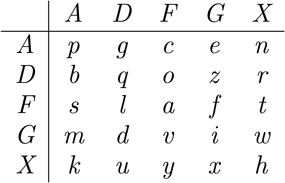
\includegraphics{UNTABLE_02_001.png}
\caption{Image taken from Trappe, Wade, and Lawrence C. Washington. Introduction to Cryptography with Coding Theory. Available from: South Dakota Board of Regents, (3rd Edition). Pearson Education (US), 2020.}
\end{figure}

\paragraph{}
From here, we take our plaintext message and create a message by mapping each 
plain text character to its corresponding row and column headers.  For example, 
in the figure above, \textit{s} is mapped to a pair, \textit{FA}.  We do this 
for every plain text character and then continue.

\paragraph{}
Next, we select our keyword and make it the column header of another matrix 
(whose width is the length of the keyword and depth determined by the length 
of the encoded message in the previous step).  We proceed by writing, from left 
to write and top to bottom, the previously encoded message into this new 
matrix until we run out of characters.

\paragraph{}
Finally, to make this cipher a bit more complex, we take the keyword header and 
order its letters alphabetically, moving the entire column associated with each 
letter as well.  Once all the columns have been reordered, we now write out the 
letters in the matrix in \textit{top to bottom, left to right} order (excluding 
the header keyword portion), giving us our encrypted message for sending.

\subsubsection{Encoding}
\paragraph{}
Before encoding, we can use a function built into the \verb|ciphers.py| module 
to get a random ordering of the alphabet, excluding the "j" character.  This is 
not strictly required for this cipher within the context of this program.  
However, if you would like to create your own seed and use it moving forward, 
the seed can be acquired using the \verb|get_random_adfgx_seed()| method, 
like so:

\begin{verbatim}
  >>> import ciphers
  >>> print(ciphers.get_random_adfgx_seed())
  zlcwetugvormnqpsbxahdkiyf
\end{verbatim}

\paragraph{}
Any random alphabet ordering, excluding "j", can be used as the initial "seed" 
for the ADFGX cipher.  Moving forward, we will simply exclude 
this parameter, as both the \verb|adfgx_encode()| and \verb|adfgx_decode()|
methods have a default parameter that is used for the seed (it happens to be 
the one shown above, \textbf{zlcwetugvormnqpsbxahdkiyf}). 

\paragraph{}
To encode, the plain text and the chosen keyword are the two parameters 
required (the third parameter is your seed, if desired).  The 
\verb|adfgx_encode()| method handles the encoding, like so:

\begin{verbatim}
  >>> import ciphers
  >>> encrypted = ciphers.adfgx_encode("Hello World!", "encrypt")
  >>> print(encrypted)
  axagdfxdaddaxadaxagx
\end{verbatim}

\paragraph{}
This sequence of commands gives us an encryption for \verb|"Hello World!"| 
using the key \verb|"encrypt"| and the default seed mentioned above.  The 
ADFGX encryption/encoding is \verb|axagdfxdaddaxadaxagx|.

\paragraph{}
Optionally, if you wish to specify your own chosen seed, you would include 
that seed as the third parameter, like so:

\begin{verbatim}
  >>> encrypted = ciphers.adfgx_encode("Hello World!", "encrypt", my_chosen_seed)
\end{verbatim}

\subsubsection{Decoding}
\paragraph{}
With knowledge of the key and the seed, decoding can be done with a little 
work behind the scenes.  Namely, because the columns were alphabetically 
reordered and some columns will not contain the same number of rows of 
characters, there is some up-front "accounting" work that must take place to 
assign variable-length blocks of the encoded message to their correct keyword 
character.

\paragraph{}
At a high level, this is achieved by taking the length of the encoded message 
and dividing it by the length of the known key.  If there is no remainder after 
the division, we can jump straight to ordering the characters in the key 
alphabetically and assigning equal blocks of the encryption to each keyword 
character.  From there, we essentially perform the exact same steps from 
encryption in reverse, eventually arriving at the decoded message.

\paragraph{}
If, however, we end up with a remainder after dividing the encoded message 
length by the keyword length, we must essentially walk through each encrypted 
letter in its original order and assign the quotient amount to each, 
\textit{then} walk back through each and add 1 to its character count until we 
reach the encrypted message length.  With this step complete, 
we can then reorder the keyword alphabetically, preserving the character count 
for each that we just assigned, and proceed to assign the respective number of 
characters from the encoded text to each respective keyword character.  
Finally, the front-end "accounting" work is complete, and we proceed with the 
decoding like in the first case.

\paragraph{}
All of this accounting work is handled in the program, saving the user the 
unnecessary headache.  Whew!  Now, to decode a message, you can use the 
\verb|adfgx_decode()| function, which takes the encrypted message, the known 
keyword, and optionally your seed as parameters, like so (using our 
\textit{Hello World!} encryption from the previous example):

\begin{verbatim}
  >>> decrypted = ciphers.adfgx_decode(encrypted, "encrypt")
  >>> print(decrypted)
  helloworld
\end{verbatim}

\paragraph{}
Again, if you wish to specify a seed other than the default stored in this 
program, you would need to add that as a third parameter in the 
\verb|adfgx_decode()| method.  Keep in mind that if you specified a seed 
other than the default in the encryption step, you \textit{must} use that 
same alternative seed in the decode step.  If you do not, you will almost 
certainly get a decrypted message that is utter nonsense.  You've been 
warned! 

%HILL CIPHER
%==============================================================================

\subsection{Hill Cipher}
\subsubsection{Description}
\paragraph{}
The Hill cipher, named after Lester Hill, is a type of block cipher.  Block 
ciphers are ciphers which perform encryption on whole "blocks" of the plain 
text, rather than on each character independently.  Most of the most effective 
ciphers used today are a derivation of a block cipher, because block ciphers 
are generally less susceptible to statistical cryptoanalysis, such as character 
frequency counting.

\paragraph{}
With the Hill Cipher, specifically, we first form an $n \times n$ matrix and fill it 
with numbers mod 26 (you could imagine these as letters mapped to numbers, if 
you wish).  This matrix serves as the \textit{key} for the cipher.  Once you 
have your key, you then section out the plain text into $n$ sized "blocks" - 
filling the last block with "x"s if needed to create a block of size $n$ - and 
perform vector/matrix multiplication between each block and 
the key, forming the cipher text.

\paragraph{}
Decoding the Hill cipher requires finding the inverse of the key matrix and 
multiplying $n$ sized blocks of the cipher text by this inversed matrix, 
ultimately yielding the original plaintext (with potentially a few "x"s at the 
tail end of the message).

\paragraph{}
Mathematically, we are performing the following calculation to encode:

Let $p_i$ be a block of plain text of length $n$.  Let $y$ be the length 
of the plaintext (padded such that $y = nk$, where $k \ge 1$).  Therefore, 
$i = 1$\ldots$(y/n)$.

Next, let the key be an $n \times n$ matrix, where each entry in the matrix 
is a number, $z$, such that $0 \le z < 26$.

Perform the following calculation for all $p_i$, $1 \le i \le (y/n)$:

$$
\begin{pmatrix}
  a_0 & a_1 & \ldots & a_n
\end{pmatrix}
_{p_i} \times
\begin{pmatrix}
  x_{0,0} & x_{0,1} & \ldots & x_{0,n}\\
  x_{1,0} & x_{1,1} & \ldots & x_{1,n}\\
  . \\
  . \\
  . \\
  x_{n,0} & x_{n,1} & \ldots & x_{n,n}
\end{pmatrix}
=
\begin{pmatrix}
  a_0 & a_1 & \ldots & a_n
\end{pmatrix}
_{c_i}
$$

\ldots where $a$ is an alphabetic character (mapped to an integer mod 26), 
$p_i$ is the plaintext vector, and $c_i$ is the resulting ciphertext vector.

\paragraph{}
Likewise, for decoding we are performing the calculation in reverse, using the 
inverse of the key matrix:

$$
\begin{pmatrix}
  a_0 & a_1 & \ldots & a_n
\end{pmatrix}
_{c_i} \times
\begin{pmatrix}
  x_{0,0} & x_{0,1} & \ldots & x_{0,n}\\
  x_{1,0} & x_{1,1} & \ldots & x_{1,n}\\
  . \\
  . \\
  . \\
  x_{n,0} & x_{n,1} & \ldots & x_{n,n}
\end{pmatrix}
^{-1} =
\begin{pmatrix}
  a_0 & a_1 & \ldots & a_n
\end{pmatrix}
_{p_i}
$$

\subsubsection{Encoding}
\paragraph{}
Like the ADFGX cipher, before encoding we can use a function to generate 
a random key for the cipher.  This is done using the 
\verb|get_random_hill_key()| method, like so:

\begin{verbatim}
  >>> import ciphers
  >>> key = ciphers.get_random_hill_key(3)
  >>> print(key)
  [[12, 15, 0], [24, 23, 15], [3, 16, 4]]
\end{verbatim}

\paragraph{}
For this method, we must pass in the block size as the one and only parameter 
(we chose $3$ here).  What we received in return is an $3 \times 3$ matrix 
that looks like this:

$$
\begin{pmatrix}
  12 & 15 & 0 \\
  24 & 23 & 15 \\
  3 & 16 & 4
\end{pmatrix}
$$

\paragraph{}
If we wanted to, we could of course represent this matrix mapped as alphabetic 
characters:

$$
\begin{pmatrix}
  m & p & a \\
  y & x & p \\
  d & q & e
\end{pmatrix}
$$

\paragraph{}
Representing the matrix either way works conceptually.  If, for example, we 
wanted to use a 9-character long keyword to fill the matrix from left to right, 
top to bottom (such as the word \textit{encrypted}, for example), this might be 
an easy way to memorize the key for both a sender and reciever.  However, 
for this program \textbf{it is required} that you provide an $n \times n$ 
matrix containing numbers mod 26.  Placing characters (not digits) into your 
key or providing numbers less than 0 or greater than or equal to 26 will throw 
an error at you.

\paragraph{}
When crafting keys, it must also be kept in mind that the matrix \textit{must} 
have a certain determinant, 
in order that it may be used for decryption.  Specifically, the determinant of 
the matrix must be the set of integers such that $gcd(det(M),26) = 1$.  If you 
plan on providing your own matrix as the Hill cipher key, you can check that it 
meets this requirement by running it through the \verb|is_valid_hill_key()| 
method, found in the \verb|ciphers.py| module, like so:

\begin{verbatim}
  >>> import ciphers
  >>> key = ciphers.get_random_hill_key(3)
  >>> print(key)
  [[12, 15, 0], [24, 23, 15], [3, 16, 4]]
  >>> print(ciphers.is_valid_hill_key(key))
  True
\end{verbatim}

\paragraph{}
Here, you can see that the random matrix retrieved by calling the 
\verb|get_random_hill_key()| method is in fact a valid key of the correct 
shape and has a valid determinant.  This is always the case 
when invoking the \verb|get_random_hill_key()| method, as it has checks built into it, 
ensuring that it will be valid.  However, if you handed it a matrix with either 
a nonsymmetrical shape or a bad determinant, it will let you know:

\begin{verbatim}
  >>> print(ciphers.is_valid_hill_key([1,2,3]))
  False
  >>> print(ciphers.is_valid_hill_key([[0,0,0],[0,0,0],[0,0,0]]))
  False
\end{verbatim}

\paragraph{}
Once we have either come up with (and checked) or generated a key for the 
cipher, we can then 
proceed to encode a plaintext message using the \verb|hill_encode()| method, 
like so (using the last randomly generated \textit{key} from the previous 
examples):

\begin{verbatim}
  >>> encrypted = ciphers.hill_encode("Hello World!", key)
  >>> print(encrypted)
  fjaohmlxnhgv
\end{verbatim}

\paragraph{}
The Hill cipher encryption using our $3 \times 3$ generated key came out 
\verb|fjaohmlxnhgv|.  Like the ADFGX cipher, \textit{key} has a built in 
default $3 \times 3$ matrix which just so happens to be the one randomly 
generated in the previous examples.  So, we could have omitted it above, 
like so:

\begin{verbatim}
  >>> encrypted = ciphers.hill_encode("Hello World!")
  >>> print(encrypted)
  fjaohmlxnhgv
\end{verbatim}

\paragraph{}
During decoding, we will need the same key we encrypted with; so, for brevity, 
the \textit{key} parameter will be omitted and the default used moving forward.

\subsubsection{Decoding}
\paragraph{}
With key in hand (or using the default, like we have been), you can decode by 
simply calling the \verb|hill_decode()| method.  Assuming we pick up where we 
left off in our last example, and we are using the default key, decoding can be 
achieved using the following commands:

\begin{verbatim}
  >>> decrypted = ciphers.hill_decode(encrypted)
  >>> print(decrypted)
  helloworldxx
\end{verbatim}

\paragraph{}
Just like that, we have decoded our \textit{Hello World!} message by 
calling the \verb|hill_decode()| method.  As mentioned at the beginning of 
this section, we have to pad any plaintext with "x"s when the length of the 
plaintext is not congruent to 0 mod26 (leaves no remainder after division).  
That explains why \verb|helloworldxx| has two pesky "x"s at the end of it!

%%%%%%%%%%%%%%%%%%%%%%%%%%%%%%%%%%%%%%%%%%%%%%%%%%%%%%%%%%%%%%%%%%%%%%%%%%%%%%%
% BASIC NUMBER THEORY
%%%%%%%%%%%%%%%%%%%%%%%%%%%%%%%%%%%%%%%%%%%%%%%%%%%%%%%%%%%%%%%%%%%%%%%%%%%%%%%

\section{Basic Number Theory}

%GCD
%==============================================================================

\subsection{GCD}
\subsubsection{Description}
\paragraph{}
Throughout almost every module and method used throughout this project, there 
has been a need to calculate the GCD, or \textit{Greatest Common Divisor}.  The 
GCD is precisely what it is says it is - the largest integer (positive or 
negative) by which two numbers can both be divided.

\paragraph{}
A trivial example would be finding the GCD of two of the same integers, like 
27 and 27, for example.  The GCD of two identical integers is always just the 
integer itself, because both 27 and 27 can be divided by 27, yielding 1!  A 
non-trivial example would be something like GCD(27,12).  Here, by a brief 
examination, we can determine that the answer is 3.  That is to say, that 3 is 
the largest integer that can divide both 27 \textit{and} 12.

\paragraph{}
In my code, finding the GCD of two integers is done using the Euclidean 
division algorithm.  This algorithm can be expressed by the following:

Let $a$ be the first integer and $b$ be the second integer.  Let $q$ be the 
quotient and $r$ the remainder from division.

If $a_0 = b_0$, $a_0$ is the solution (or $b_0$, because they are equal).  Otherwise, 
let $a_0 < b_0$.

\begin{gather*}
b_0 = a_0 q_0 + r_0 \\
a_0 = q_1 r_0 + r_1 \\
q_1 = q_2 r_1 + r_2 \\
. \\
. \\
. \\
q_{n-1} = q_n r_{n-1} + 0
\end{gather*}

Proceed reducing the above equations solving for $q$ and $r$ on the right 
hand side of the equation until $r_n = 0$.  When $r_n = 0$, the GCD is given 
by $q_n$.

\subsubsection{Using the Method}
\paragraph{}
Much like the previous section of this document, we can use the Python REPL to 
execute and test out this method.  Here are some basic examples of the method 
in action:

\begin{verbatim}
  >>> import cryptomath
  >>> print(cryptomath.gcd(102,16))
  2
\end{verbatim}

\paragraph{}
Here we see that by calling \verb|cryptomath.gcd(102,16)|, we receive 
\verb|2| as our answer.  By observation, we should see that this is in fact 
correct.  We can try a few more examples just to demonstrate:

\begin{verbatim}
  >>> print(cryptomath.gcd(102,17)) 
  17
  >>> print(cryptomath.gcd(102,102)) 
  102
  >>> print(cryptomath.gcd(-1,1))    
  -1
  >>> print(cryptomath.gcd(-1,0)) 
  -1
  >>> print(cryptomath.gcd(-1,-12)) 
  1
\end{verbatim}

\paragraph{}
As can be seen above, using negative integers and zero are also acceptable 
parameters for the method.  Passing $1$ or $-1$ as a parameter will 
\textit{always} yield a $1$ or $-1$ and passing $0$ will always return the 
other parameter as an answer.  Why should be apparent to even the most casual 
reader.

%EXTENDED GCD
%==============================================================================

\subsection{Extended GCD}
\subsubsection{Description \& Use}
\paragraph{}
The \verb|extended_gcd()| method included in this program solves for $x$ and 
$y$ in the Diophantine equation $ax + by = c$.  To solve this, we start by 
first performing the Euclidean division algorithm as in the previous step.  
However, instead of solving until we reach $r_n = 0$, as in the previous step, 
we must stop the division when we reach $r_n = 1$.  Working "backwards" from 
this point, we can eventually arrive at the general Diophantine equation 
$ax + by = 1$.  The method ultimately returns both the $x$ and $y$ variables 
to the caller.

\paragraph{}
To demonstrate, we can call the method like so:

\begin{verbatim}
  >>> print(cryptomath.extended_gcd(3,17)) 
  (6, -1)
  >>> print(cryptomath.extended_gcd(101,14)) 
  (5, -36)
\end{verbatim}

\paragraph{}
As you can see, the method returns a pair of integers, $x$ and $y$ that 
correspond to the coefficients $a$ and $b$ passed in, such that the general 
Diophantine equation $ax + by = 1$ is solved.  Switching the order of $a$ and 
$b$ in the parameter list will switch the returned $x$ and $y$ pair, 
respectively, like so:

\begin{verbatim}
  >>> print(cryptomath.extended_gcd(17,3))
  (-1, 6)
  >>> print(cryptomath.extended_gcd(3,17)) 
  (6, -1)
\end{verbatim}

\subsubsection{Considerations}
\paragraph{}
As a final note, you must keep in mind that a Diophantine equation where the 
coefficients $a$ and $b$ have $gcd(a,b) \neq 1$ yields multiple solutions!  As 
such, the program will raise an Exception should you pass it parameters $a$ and 
$b$ not meeting this condition:

\begin{verbatim}
  >>> print(cryptomath.extended_gcd(7,14))   
  Traceback (most recent call last):
    .
    .
    .
  cryptomath.InfiniteSolutionsException: No single solution can be arrived
  at for extended_gcd(a,b).
\end{verbatim}

%FINDING MODULAR INVERSE
%==============================================================================

\subsection{Finding Modular Inverse}
\subsubsection{Description}
\paragraph{}
Sometimes in modular arithmetic we are faced with a predicament.  Let's say, 
for example, that we want to solve for $x$ in the equation $9x = 3 mod(7)$. If 
we were to divide the coefficient $9$ from both sides, we would arrive at the 
equation $x = \frac{1}{3} mod(7)$.  However, we are typically used to dealing 
strictly with integers in modular arithmetic.  What does $\frac{1}{3} mod(7)$ 
even mean?

\paragraph{}
Well, in fact the meaning of $9x = 3 mod(7)$ was better understood before 
having simplified to $x = \frac{1}{3} mod(7)$.  What $9x = 3 mod(7)$ is really 
saying is that there is an integer $x$ such that when multiplied by $9$ will 
give us a result that is 3 more than some number $y$, multiplied by $7$.  In 
mathematical terms, we could express this as $9x = 7y + 3$.  When expressed 
this way, we find that what we are looking at is really just a Diophantine 
equation, $9x - 7y = 3$.  By reframing the problem in this way, we can simply 
use our \verb|extended_gcd()| method from before to find $x$, and we have 
solved an otherwise seemingly difficult problem.

\subsubsection{Using the Method}
\paragraph{}
To solve for the equation from the description above, $9x = 3 mod(7)$, we begin 
by arranging the equation into the unfamiliar form from before, 
$x = \frac{1}{3} mod(7)$.  Once in this form, let $a = 3$, or the denominator 
of the fraction $\frac{1}{3}$; and let $n = 7$, or the modulus we are working 
within for the problem.  To find the solution for $x$, we can use the 
\verb|find_modular_inverse()| method in the \verb|cryptomath.py| module by 
passing in the values for $a$ and $n$, like so:

\begin{verbatim}
  >>> import cryptomath
  >>> print(cryptomath.find_mod_inverse(3,7))
  5 
\end{verbatim}

\paragraph{}
We can see that the solution is $x = 5$.  We can verify that this is in fact 
the case through mere observation: $9*5 = 45$ and $45 - 3 = 42$, which is a 
multiple of $7$ ($7*6 = 42$).

\subsubsection{Considerations}
\paragraph{}
What happens if we don't end up with a seemingly "nice" fraction like 
$\frac{1}{3}$?  Recall from the description and considerations of 
\textit{Extended GCD} that we are typically solving the \textit{general} 
Diophantine equation, $ax + by = 1$.  This all works nicely when the numerator 
of our fraction is $1$, but what about when the numerator is greater than $1$?

\paragraph{}
If we happen to be in a situation where we need to solve something like 
$x = \frac{4}{5} mod(7)$, we don't need to fear!  We are able to multiply the 
numerator of our fraction, $\frac{4}{5}$ by the result, $x$, to achieve the 
answer.  Using $x = \frac{4}{5} mod(7)$, where our $a = 5$ and our $n = 7$, we 
can invoke the method to get the first part of our answer, like before:

\begin{verbatim}
  >>> import cryptomath
  >>> print(cryptomath.find_mod_inverse(5,7))
  3
\end{verbatim}

\paragraph{}
The method returned the result $x = 3$.  However, we can see from mere 
observation that $5*3 = 15 \neq 4 mod(7)$.  We must perform one last step and 
multiply the numerator from our fraction, $4$, by the method's result to get 
the actual answer, $4*3 = 12$.  Checking that this is in fact correct, 
$5*12 = 60 = 4 mod(7)$.

%FINDING MODULAR INVERSE OF A MATRIX
%==============================================================================

\subsection{Finding Modular Inverse of a Matrix}
\subsubsection{Description}
\paragraph{}
Matrices are much like integers in that we can place them within the bounds of 
modular math.  Recall, that the Hill Cipher from Section 2.6 used matrices to 
encrypt messages, and that the key for the Hill Cipher had to have integers that 
were no less than 0, but also no greater than 25.  This is the same as saying 
that the Hill Cipher requires some matrix, $M mod(26)$.

\paragraph{}
Much like the problem we faced in the previous section where we ended up with 
a fraction on the right hand side of our modular equation, when performing matrix 
operations under modular bounds, we can sometimes wind up in a situation where 
we have fractions in a matrix that need to be converted to their modular 
inverses to make sense.  As a matter of fact, we can recall that during the 
decoding step of the Hill Cipher, we had to multiply by the inverse of the key. 
If we simply took the inverse of any Hill Cipher key, we almost certainly end 
up with a matrix containing all sorts of ugly fractions - fractions that we 
subsequently need to convert to their modular inverses to use in a meaningful 
way.  The \verb|inverse_matrix_modular()| method does just that.

\subsubsection{Using the Method}
\paragraph{}
To use \verb|inverse_matrix_modular()|, we must pass the method a 
$n \times n$ matrix and (optionally) the modulus we are working in, like so:

\begin{verbatim}
  >>> import cryptomath
  >>> matrix = [[7, 8, 13], [25, 2, 2], [1, 25, 19]]
  >>> print(cryptomath.inverse_matrix_modular(matrix))
  [[24, 5, 20], [23, 20, 15], [15, 9, 8]]
\end{verbatim}

\paragraph{}
If we exclude the modulus we want to work in, it defaults to $mod(26)$.
In the example above, the method returns us the inverse matrix of the original 
matrix mod(26).

\subsubsection{Considerations}
\paragraph{}
There are two considerations when using this method.  First, the 
matrix you construct \textit{must be} invertible; and secondly, it must also
have a modular inverse to begin with.  These two considerations place somewhat 
strict boundaries on what constitutes acceptable input for the method.  As a 
matter of fact, for the demonstration above, the matrix I chose was \textit{not} 
chosen at random.  This matrix met both of these restrictions and was actually 
constructed using the \verb|get_random_hill_key()| method from Section 2.6, 
which does a fair amount of prelimary checking to ensure that the Hill Cipher 
key it gives you is valid.

\paragraph{}
For first-time users of this method, I would encourage the use of the 
\verb|get_random_hill_key()| method to construct your input matrix.

%PRIMALITY TEST
%==============================================================================

\subsection{Primality Test}
\subsubsection{Description}
\paragraph{}
For many cryptographic systems and cryptoanalysis techniques, it is useful to 
be able to calculate the primality of a number (whether or not it is prime or 
composite).  In the \verb|cryptomath.py| module included with this project, 
there is a method dedicated to this task.  The method included uses the 
"Miller-Rabin" primality test to help deal with very large primes.

\paragraph{}
The Miller-Rabin primality test (as implemented here) can be described by the 
following algorithm:

\begin{algorithm}
	\begin{algorithmic}
    \State Let integer $n > 1$ and be odd.
    \State Calculate $k$ and $m$ such that $n - 1 = 2^{k}m$ and $m$ is odd.
    \State Let $b_{i} = 2^{m} \mod{n}$ and $i = 0$
    \If {$b_{i} = \pm 1 \mod{n}$}
      \State $n$ is likely prime
    \EndIf
    \For {$iterator=k,(k-1),(k-2),\ldots, 2$}
      \State $i = i + 1$
      \State $b_{i} = b_{i-1}^{2} \mod{n}$
      \If {$b_{i} = 1$}
        \State $b$ is composite
      \ElsIf {$b_{i} = n-1$}
        \State $b$ is likely prime
      \EndIf
    \EndFor
	\end{algorithmic} 
\end{algorithm}

\paragraph{}
If the entire algorithm executes without ever determining either composite or 
prime explicitly, the method returns \textbf{False}, indicating that we assume 
the number $b$ is not prime.  Notice that the Miller-Rabin primality test does 
not make the claim of being able to determine with \textit{absolute certainty} 
that a number is prime - thus the phrase, "\textit{$b$ is likely prime}", not 
"\textit{$b$ is prime}".

\subsubsection{Using the Method}
\paragraph{}
To use the \verb|is_prime()| method, we simply pass the number into the method 
that we wish to test for prime, like so:

\begin{verbatim}
  >>> import cryptomath
  >>> print(cryptomath.is_prime(101))
  True
\end{verbatim}

\paragraph{}
Here, we see that passing the method $101$, which we know is a prime number, 
will return \textbf{True}, indicating that it is in fact prime.  We could also 
try some other numbers to illustrate further:

\begin{verbatim}
  >>> print(cryptomath.is_prime(105)) 
  False
  >>> print(cryptomath.is_prime(740)) 
  False
  >>> print(cryptomath.is_prime(1901)) 
  True
\end{verbatim}

\paragraph{}
In these examples, we started with two numbers that we know just from observation 
are composite, $105$ (divisible by 5) and $740$ (even, or divisible by 2).  
Finally, we passed the method $1901$, which it determined is \textit{likely} 
prime.  A quick search online can verify that, in fact, $1901$ is a known 
prime.

\subsubsection{Considerations}
\paragraph{}
The \verb|is_prime()| method included has not been thoroughly stress tested to 
determine it's upper limits.  Initially, the method had trouble handling some 
integers that were only in the 4-digit range.  To solve this issue, an 
underlying iterative method was constructed to break large values of $m$ (from 
the Miller-Rabin algorithm above) into manageable pieces and merge them to find 
results mod(n).  This allowed the method to stretch considerably;
however, as the tested integer grows, so does the time needed to compute the 
primality.

\paragraph{}
Currently, the method can handle up to 8-digit numbers with virtually no lag 
or delay.  9-digit numbers will register a very short delay.  10-digit numbers 
will register a noticeable delay (but, not unbearable).  As mentioned, no 
considerable stress testing or timed testing has been performed yet, so the 
user should expect unknown delays in computation when trying to test the 
primality of very large integers.

%GENERATING A RANDOM PRIME
%==============================================================================

\subsection{Generating a Random Prime}
\subsubsection{Description and Use}
\paragraph{}
Much like finding a prime number, generating a random prime number is often 
required in cryptographic systems.  In particular, the RSA algorithm 
requires the ability to generate two large random primes and multiply 
them together to create a public key (a very large, very hard to factor, 
composite number).

\paragraph{}
The method used here to generate random prime numbers relies on our previously 
covered \verb|is_prime()| method.  To generate a prime, we must determine 
approximately what order of magnitude we want our prime.  Specifically, we will 
pass the method a value, $b$, such that the prime number we want is within the 
range $2^{b} - 1 \le b \le 2^{b+1} - 1$, like so:

\begin{verbatim}
  >>> import cryptomath
  >>> my_prime = cryptomath.random_prime(10)
  >>> print(my_prime)
  1069
\end{verbatim}

\paragraph{}
We can verify that, in fact, $1069$ is prime (by looking online) and that it 
meets the criteria $2^{10} - 1 \le 1069 \le 2^{11} - 1$.

\subsubsection{Considerations}
\paragraph{}
Because this method relies on the \verb|is_prime()| method, it is subject to 
the limitations inherited from \verb|is_prime()| - namely, that for 
$b \ge 29$ we should 
expect some delay (depending on our machine, of course).  

\paragraph{}
Also, it should be 
noted that when we get into the order of magnitude where $b \ge 29$, the 
expected delays are not predictable.  There are times at which we may 
experience substantial delays, and other times where the delays may be 
relatively short.  This is a function of the fact that the algorithm used 
actually picks a random number, $r$, within $2^b - 1 \le r \le 2^{b+1} - 1$, 
tests it for 
prime, and if not prime, loops back and tries again.  If the algorithm happens 
to choose a prime number in short order, the delay may be bearable.  If the 
algorithm continuously picks composite numbers, the delay may be excruciating.

%FACTORING A COMPOSITE
%==============================================================================

\subsection{Factoring a Composite}
\subsubsection{Description}
\paragraph{}
Much like the previous section where we wanted to be able to generate large 
primes, we often also want to be able to factor large composites.  As a matter 
of fact, determining better ways to factor very large composite numbers is the sole focus of 
entire studies, academic papers, and organizations.  The usefulness and 
security of the RSA encryption scheme entirely depends on the fact that 
extracting one (or both) of the two large factors that are used to generate 
the composite public key is too computationally expensive - even for the best 
machines on the market today.  Exposing the public key poses virtually no risk 
to the security of RSA precisely because factoring is so difficult.

\paragraph{}
The method used for factorization in this program, \verb|factor()|, allows the 
user to choose from three well-known factorization methods:  Fermat's method, 
the Pollard-Rho method, and the Pollard "p-1" method.  A brief description of 
each algorithm follows.

\paragraph{Fermat's Method}
Fermat's method is the oldest (and consequently, least efficient) of the three.  
The algorithm can be summed up by the following pseudocode:

\begin{algorithm}[H]
	\begin{algorithmic}
    \State Let $n$ be a large composite number
    \State $y \gets 1$
    \State $x \gets n + y^2$
    \While{$x$ not a perfect square and $y < \sqrt{n}$}
      \State $y \gets y + 1$
      \State $x \gets n + y^2$
    \EndWhile
    \If{$x$ is a perfect square}
      \State $factor1 = \sqrt{x} - y$
      \State $factor2 = \sqrt{x} + y$
    \Else{}
      \State Failed to factor $n$
    \EndIf
	\end{algorithmic} 
\end{algorithm}

\paragraph{}
As can be observed from the algorithm, the relative efficiency of calculating 
the factors for $n$ is primarily dependent on how far apart the two factors are 
from one another.  For two factors that reside close to one another (for cases 
where $y$ is small), the algorithm can execute very quickly.  However, as the 
distance between the two factors grows, so does the execution time.  For very 
large composites, this means Fermat's method could be slow in comparison to 
other methods.

\paragraph{Pollard Rho}
The Pollard-Rho algorithm was invented by John Pollard in 1975.  The algorithm 
performs much better than Fermat's factorization algorithm on average.  There are 
various implementations of the algorithm, however all of them utilize the same 
basic premise.

\paragraph{}
The algorithm relies on and takes advantage of the fact that under modular 
arithmetic, we can expect to "loop back" through the modular field after so 
many iterations, or after large operations on the same value, such as 
exponentiation.  The implementation used in this program also relies on 
some randomization as well.  The algorithm is summarized as follows:

\begin{algorithm}[H]
	\begin{algorithmic}
    \State Let $n$ be a large composite number
    \State $d \gets 1$
    \State Let $g(s) = (s^2 + 1) \mod{n}$
    \While{$d = 1$ or $d = n$}
      \State Let $r1$ be random integer such that $1 \le r1 < n$
      \State Let $r2$ be random integer such that $1 \le r2 < n$
      \State $x \gets g(r1)$
      \State $y \gets g(g(r2))$
      \State $d \gets GCD(|x - y|, n)$
    \EndWhile
    \If{$d \neq 1$}
      \State $factor1 = d$
      \State $factor2 = n/d$
    \Else{}
      \State Failed to factor $n$
    \EndIf
	\end{algorithmic} 
\end{algorithm}

\paragraph{}
As can be observed from the algorithm above, there is no guarantee that the 
while loop will actually terminate in this implementation.  If $n$ is not 
actually composite, for example, this algorithm would never terminate!

\paragraph{Pollard p-1}
The year before the Pollard-Rho algorithm was invented by Pollard, he had 
invented a different algorithm titled "p-1".  This algorithm is very effective 
under special circumstances:  namely, when one of the factors of $n$, $p$, has 
the property that $p-1$ only has relatively small prime factors.  While having 
this special property may seem like it narrows the usefulness of the algorithm, 
it turns out that the Pollard "p-1" algorithm is actually quite effective in 
the general - still beating out Fermat's on average.

\paragraph{}
The implementation of the "p-1" algorithm for this program is given by the 
following pseudocode:

\begin{algorithm}[H]
	\begin{algorithmic}
    \State Let $n$ be a large composite number
    \State Let $B$ be a random integer such that $1 < B < n$
    \State $d \gets 1$
    \While{$B > 0$ and $d = 1$ or $d = n$}
      \State $p \gets b^B \mod{n}$
      \State $B \gets B - 1$
      \State $d \gets GCD(p-1, n)$
    \EndWhile
    \If{$d \neq 1$}
      \State $factor1 = d$
      \State $factor2 = n/d$
    \Else{}
      \State Failed to factor $n$
    \EndIf
	\end{algorithmic} 
\end{algorithm}

\subsubsection{Using the Method}
\paragraph{}
To use the \verb|factor()| method included with this program, we must pass the
method our composite number, $n$, and a flag, $m$, indicating which method we 
would like to use for factorization: "f" indicates we want to use Fermat's 
method; "r" indicates Pollard-Rho; and "p" indicates Pollard "p-1".  Here's 
an example of invoking the method in the REPL:

\begin{verbatim}
  >>> import cryptomath
  >>> print(cryptomath.factor(31664593,"f"))
  (4297, 7369)
\end{verbatim}

\paragraph{}
Here, the method used Fermat's method to factor \textbf{31664593} into two 
prime factors, \textbf{4297} and \textbf{7369}.  Note:  This 
large composite was calculated ahead of time to ensure that it was factorable.  
If this large number had been prime, the method would have thrown an Exception, 
like so:

\begin{verbatim}
  >>> print(cryptomath.factor(45774107,"f")) 
  Traceback (most recent call last):
    .
    .
    .
  cryptomath.FactoringException: Factoring method was passed a prime or 
    incorrect flag.
\end{verbatim}

\paragraph{}
Using either of the other two factorization methods is done in an identical 
way; simply pass "r" or "p", instead of "f".  The flag, $m$, is technically 
a default parameter and is not necessary.  If you choose to omit the flag, 
the method will default to using the Pollard-Rho factorization method.


%%%%%%%%%%%%%%%%%%%%%%%%%%%%%%%%%%%%%%%%%%%%%%%%%%%%%%%%%%%%%%%%%%%%%%%%%%%%%%%
% DATA ENCRYPTION STANDARD
%%%%%%%%%%%%%%%%%%%%%%%%%%%%%%%%%%%%%%%%%%%%%%%%%%%%%%%%%%%%%%%%%%%%%%%%%%%%%%%

\section{Data Encryption Standard}
\subsection{Simplified DES}
\subsubsection{Overview}
\paragraph{}
The Data Encryption Standard, or DES for short, is a symmetric-key block cipher 
historically used for the encryption of data.  The DES has a 56-bit key length, 
which, by today's standards, is too short to be considered secure.  Today, most 
block ciphers are using either 128-bit, 192-bit, or 256-bit encryption keys, 
along with other improvements that make them secure enough to be trusted by 
banking, government, and commercial institutions.

\paragraph{}
For this project, I have implemented a simplified version of the DES.  In this 
simplified version, blocks are only 12-bits, rather than 64-bits.  The simplified 
DES only implements 4 rounds by default, unlike the standard DES which has 16 
rounds.  Finally, the simplified version here has only 2-boxes to standard DES' 
8; and each simplified S-box has two rows with 8 columns each, versus the standard DES 
with it's 4 rows, 16 columns per S-box.  The simplified DES key can be variable 
length; however, it's guaranteed that only the first 9 bits of
the key will actually be used during encryption.

\subsubsection{Encryption}
\paragraph{}
To encrypt with the simplified DES, you can call the \verb|simplified_encrypt()| 
method in the \verb|des.py| module, passing in the plaintext you'd like to 
encrypt, along with a key of your choice, and optionally the number of rounds 
you'd like to have the algorithm go through, like so:

\begin{verbatim}
  >>> import des
  >>> ciphertext = des.simplified_encrypt("Hello World!", "encrypt", 4)
  >>> print(ciphertext)
  ÙÉYnýÃ
\end{verbatim}

\paragraph{}
You can see that the encryption for \verb|"Hello World!"| ends up being 
\verb|ÙÉYnýÃ|.  One might be curious why the number of characters shown in 
the encryption (6) are fewer in count than the number of characters passed into the 
method (12).  Is this behaving like a compression algorithm?  Not exactly.

\paragraph{}
The way I've implemented the simplified DES is by "chopping up" the plaintext 
into 12-bit blocks.  However, I assume during encryption that the characters of the 
plaintext are no wider than 8 bits in length - that is, they are within the 
ASCII character values 0 to 255.  During the last stage of encryption when these 
12-bit "chunks" are reassembled and converted back into a string (the ciphertext), 
the actual encoding of the bits is interpreted as a 16-bit wide character set 
(ASCII values 0 to 65,535).  This explains why our encryption is actually half 
the length of our encrypted plaintext - half the length in visible characters, 
not in bits!

\subsubsection{Decryption}
\paragraph{}
To decrypt the ciphertext, we can utilize the \verb|simplified_decrypt()| 
method.  This method takes the same parameters as the 
\verb|simplified_encrypt()| method - the text to decrypt, the encryption key, 
and the number of rounds (defaults to 4, if excluded) - like so:

\begin{verbatim}
  >>> decrypted = des.simplified_decrypt(ciphertext, "encrypt")
  >>> print(decrypted)
  Hello World!
\end{verbatim}

\paragraph{}
Using our ciphertext from before, we can see that passing this into the 
\verb|simplified_decrypt()| with the same encryption key as before yields 
our original plain text: \verb|Hello World!|.  Notice, that I excluded the 
parameter for the number of rounds.  When excluded for either the 
\verb|simplified_encrypt()| or \verb|simplified_decrypt()| methods, the 
default number of rounds is 4.

%%%%%%%%%%%%%%%%%%%%%%%%%%%%%%%%%%%%%%%%%%%%%%%%%%%%%%%%%%%%%%%%%%%%%%%%%%%%%%%
% RSA
%%%%%%%%%%%%%%%%%%%%%%%%%%%%%%%%%%%%%%%%%%%%%%%%%%%%%%%%%%%%%%%%%%%%%%%%%%%%%%%

\section{RSA}
\subsection{Description}
\paragraph{}
RSA is a public key cryptosystem named after it's authors Rivest, Shamir, and 
Adleman.  It was officially released/invented in 1977, however there is 
evidence that British government agencies had discovered the method 7 years 
earlier, but had kept it secret.

\paragraph{}
RSA is remarkably elegant.  So much so, that an exhaustive discussion of it is 
not really necessary here.  It relies on a simple premise that has already 
been discussed in previous sections; that is, that factoring very large 
composite numbers into two distinct primes is incredibly difficult.  Utilizing 
this fact, RSA encrypted messaging is performed using the following steps:

\begin{itemize}
  \item Person A calculates $n = pq$, where $p$ and $q$ are very large distinct 
  primes.  Person A keeps $p$ and $q$ secret, but exposes $n$ as their public 
  key.
  \item Person A calculates an encryption exponent, $e$, such that 
  $GCD(e,(p-1)(q-1)) = 1$.  This is also made public.
  \item Person A also calculates a decryption exponent, $d$, such that 
  $de = 1 \mod((p-1)(q-1))$.  \textit{This decryption exponent is kept private}.
  \item When Person B wishes to send a message to Person A, they do so by 
  encrypting their message, $m$, using the function, $E(m) = m^e \mod{n}$.
  \item Person A decrypts the recieved message using the function, 
  $D(E(m)) = E(m)^d \mod(n)$.
\end{itemize}

\paragraph{}
Again, very elegant and effective.  There is little else to it, other than the 
limitation that $n$ be larger than the message it is encrypting.  If the 
message is greater than $n$, the message can be broken up into "blocks" (just 
like they were in DES), and each "block" encrypted and decrypted independently.

\subsection{Using the Method}
\paragraph{}
To use RSA within the context of this program, we must first import the 
\verb|rsa.py| module.  From there, we can invoke either the \verb|encode()| or 
\verb|decode()| methods to encrypt or decrypt messages, respectively.

\paragraph{}
However, before jumping right into encryption, we must first calculate the $n$, 
$e$, and $d$ that were mentioned in the previous section.  To calculate $n$, we 
can call on the \verb|random_prime()| method from the \verb|cryptomath.py| 
module, like so:

\begin{verbatim}
  >>> import cryptomath
  >>> p = cryptomath.random_prime(10) 
  >>> p = cryptomath.random_prime(6)  
  >>> n = p*q    
  >>> print(n)
  15023
\end{verbatim}

\paragraph{}
Here, we see that we were able to generate two large distinct prime numbers and 
multiply them together to acquire $n$.  For now, we will want to keep $p$ and 
$q$ as well (don't forget to keep these private!), as they will be needed in 
the next step to calculate our public encryption exponent and private 
decryption exponent.

\paragraph{}
To calculate $e$ and $d$, we can invoke a method in the \verb|rsa.py| module 
called \verb|get_public_private_pair()|, like so:

\begin{verbatim}
  >>> import rsa
  >>> e, d = rsa.get_public_private_pair(p,q)
  >>> print(e)
  9973
  >>> print(d)
  37
\end{verbatim}

\paragraph{}
Here we see that the method returned to exponents, \textbf{9973} and 
\textbf{37}, which can be used for encryption and decryption, 
respectively.  Note that either $e$ or $d$ can be made the public or the 
private exponent.  Which is used as public and which is used as private does 
not matter, as long as the private one stays private!

\paragraph{}
With all of the above preliminaries out of the way, we can finally send a 
message!  If we are Person B, looking to send an RSA-encrypted message to 
Person A (assuming they've exposed $n$ and $e$ for us already), we can do so 
using the \verb|encode()| message, like so:

\begin{verbatim}
  >>> encrypted = rsa.encode("Please accept my invitation to a super secret 
    gathering tonight.", e, n)
  >>> print(encrypted)
  [5691, 4271, 9694, 11696, 3334, 9694, 5824, 11696, 6764, 6764, 9694, 3683, 
    5546, 5824, 10788, 2636, 5824, 10193, 13207, 13215, 10193, 5546, 11696, 
    5546, 10193, 14804, 13207, 5824, 5546, 14804, 5824, 11696, 5824, 3334, 389, 
    3683, 9694, 1272, 5824, 3334, 9694, 6764, 1272, 9694, 5546, 5824, 8308, 
    11696, 5546, 6981, 9694, 1272, 10193, 13207, 8308, 5824, 5546, 14804, 
    13207, 10193, 8308, 6981, 5546, 10637]
\end{verbatim}

\paragraph{}
Here we have encrypted our message and printed out the encryption.  The 
encryption is stored as "blocks" of integers.  We have quite a few blocks for 
such a short message; however, this was expected when we recall that each 
"block" must be smaller than $n$.  And here, our $n$ is relatively small.

\paragraph{}
After Person B has sent this encryption over the wire, Person A now wants to 
decrypt the message.  To do so, they can invoke the \verb|decode()| method, 
like so:

\begin{verbatim}
  >>> print(rsa.decode(encrypted,d,n))
  Please accept my invitation to a super secret gathering tonight.
\end{verbatim}

\paragraph{}
Voila!  We have decoded the invitation to the super secret gathering tonight.
Notice that for this method, we are passing in the \textit{decryption} 
exponent in place of the encryption exponent from last time.

\subsection{Considerations}
\paragraph{}
The implementation here is, admittedly, somewhat crude and has not been 
optimized to a high degree.  In the examples above, I used fairly small prime 
numbers to calculate $n$; numbers small enough that they would offer virtually 
no real security benefit in a real life application.  However, due to both 
computational limitations and limitations on time, computing very large 
(practically secure) public and private keys/exponents proved elusive within 
the context of this program.  Perhaps at a future date, the underlying methods 
used to calculate very large modular exponentiation will be streamlined, making 
this much closer to a real-world RSA!

%===========================================================
%===========================================================

\bibliographystyle{ieeetr}
\bibliography{refs}


\end{document} 